\documentclass[11pt,a4paper]{article}
\usepackage{graphicx}
\usepackage{tcolorbox}
\usepackage{xcolor}
\usepackage{geometry}
\usepackage{tikz}
\usetikzlibrary{calc}
\geometry{margin=0.8in}

% Define colors
\definecolor{mlblue}{RGB}{31, 119, 180}
\definecolor{mlorange}{RGB}{255, 127, 14}
\definecolor{mlgreen}{RGB}{44, 160, 44}
\definecolor{mlred}{RGB}{214, 39, 40}
\definecolor{mlpurple}{RGB}{148, 103, 189}

\title{\Large\textbf{Discovery 4: Distance Matters}\\
\vspace{0.3em}
\normalsize How Do You Measure ``Close''?}
\date{}

\begin{document}
\maketitle
\vspace{-2em}

\section*{Three Ways to Measure Distance}

\begin{center}
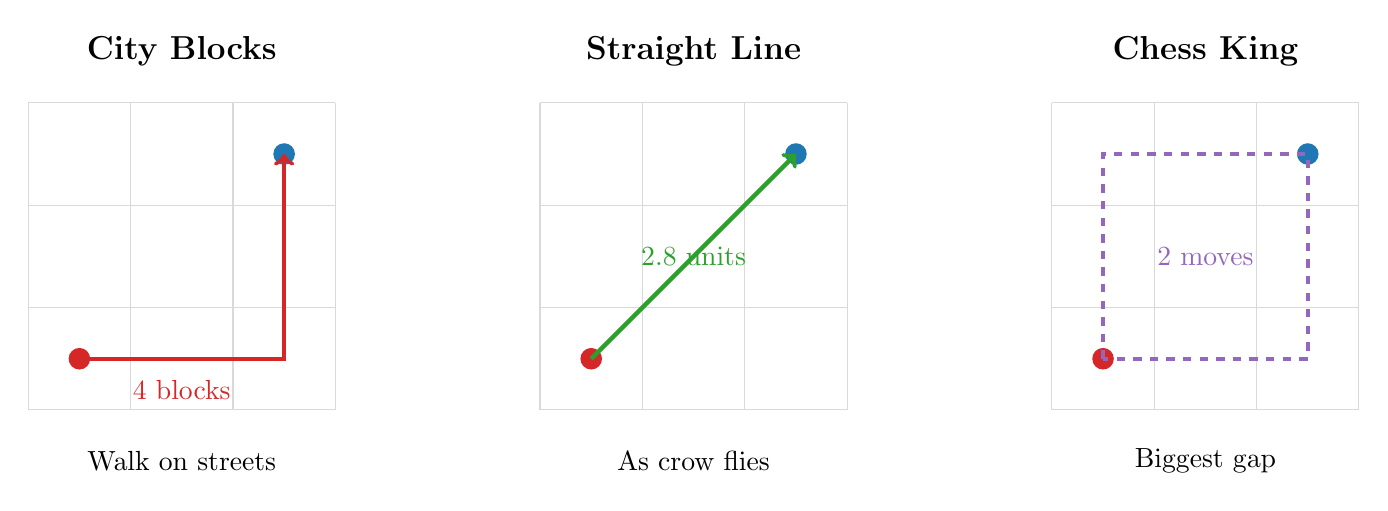
\begin{tikzpicture}[scale=1.3]
% City blocks (Manhattan distance)
\begin{scope}[shift={(0,0)}]
\draw[gray!30] (0,0) grid (3,3);
\node[font=\large\bfseries] at (1.5,3.5) {City Blocks};
\fill[mlred] (0.5,0.5) circle (3pt);
\fill[mlblue] (2.5,2.5) circle (3pt);
\draw[ultra thick, mlred, ->] (0.5,0.5) -- (2.5,0.5) -- (2.5,2.5);
\node at (1.5,-0.5) {Walk on streets};
\node[mlred] at (1.5,0.2) {4 blocks};
\end{scope}

% As the crow flies (Euclidean)
\begin{scope}[shift={(5,0)}]
\draw[gray!30] (0,0) grid (3,3);
\node[font=\large\bfseries] at (1.5,3.5) {Straight Line};
\fill[mlred] (0.5,0.5) circle (3pt);
\fill[mlblue] (2.5,2.5) circle (3pt);
\draw[ultra thick, mlgreen, ->] (0.5,0.5) -- (2.5,2.5);
\node at (1.5,-0.5) {As crow flies};
\node[mlgreen] at (1.5,1.5) {2.8 units};
\end{scope}

% Maximum difference (Chebyshev)
\begin{scope}[shift={(10,0)}]
\draw[gray!30] (0,0) grid (3,3);
\node[font=\large\bfseries] at (1.5,3.5) {Chess King};
\fill[mlred] (0.5,0.5) circle (3pt);
\fill[mlblue] (2.5,2.5) circle (3pt);
\draw[ultra thick, mlpurple, dashed] (0.5,0.5) rectangle (2.5,2.5);
\node at (1.5,-0.5) {Biggest gap};
\node[mlpurple] at (1.5,1.5) {2 moves};
\end{scope}
\end{tikzpicture}
\end{center}

\vspace{1em}

\begin{tcolorbox}[colback=mlorange!10, colframe=mlorange!50]
\centering\Large
\textbf{Same points. Different distances. Different groups!}
\end{tcolorbox}

\vspace{2em}

\section*{Your Turn: Who's Closest?}

\begin{center}
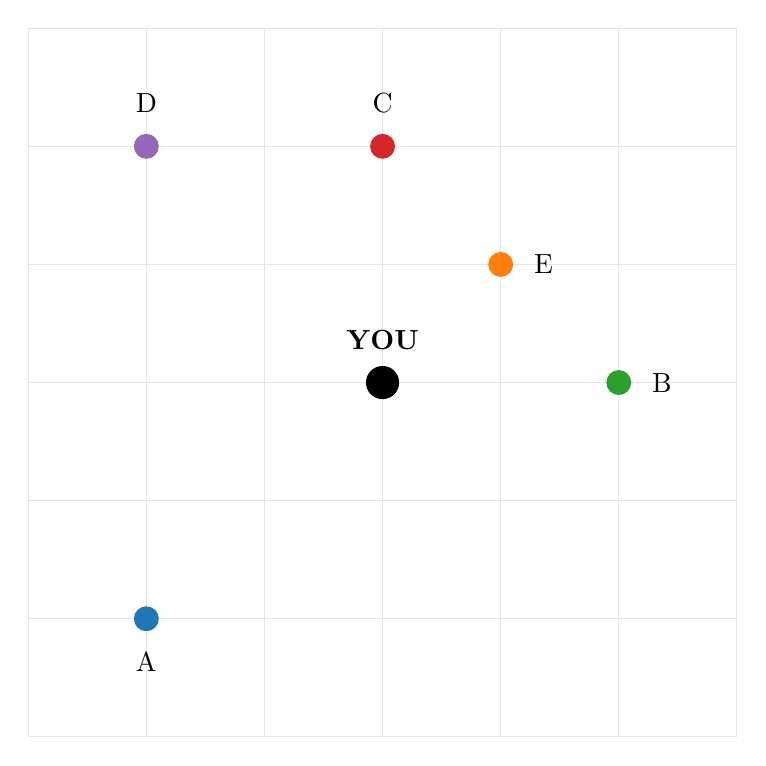
\begin{tikzpicture}[scale=1.5]
\draw[gray!20] (0,0) grid (6,6);

% Central point
\fill[black] (3,3) circle (4pt);
\node[above] at (3,3.2) {\textbf{YOU}};

% Other points
\fill[mlblue] (1,1) circle (3pt);
\node[below] at (1,0.8) {A};

\fill[mlgreen] (5,3) circle (3pt);
\node[right] at (5.2,3) {B};

\fill[mlred] (3,5) circle (3pt);
\node[above] at (3,5.2) {C};

\fill[mlpurple] (1,5) circle (3pt);
\node[above] at (1,5.2) {D};

\fill[mlorange] (4,4) circle (3pt);
\node[right] at (4.2,4) {E};
\end{tikzpicture}

\vspace{1em}

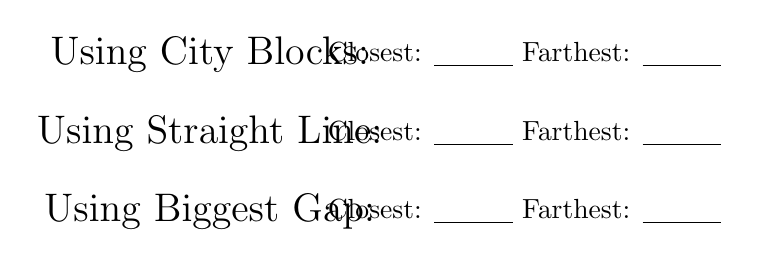
\begin{tikzpicture}[scale=1]
\node at (0,0) {\Large Using City Blocks:};
\node at (4,0) {Closest: \underline{\hspace{1cm}} Farthest: \underline{\hspace{1cm}}};

\node at (0,-1) {\Large Using Straight Line:};
\node at (4,-1) {Closest: \underline{\hspace{1cm}} Farthest: \underline{\hspace{1cm}}};

\node at (0,-2) {\Large Using Biggest Gap:};
\node at (4,-2) {Closest: \underline{\hspace{1cm}} Farthest: \underline{\hspace{1cm}}};
\end{tikzpicture}
\end{center}

\newpage

\section*{Real World: When Distance Type Matters}

\begin{center}
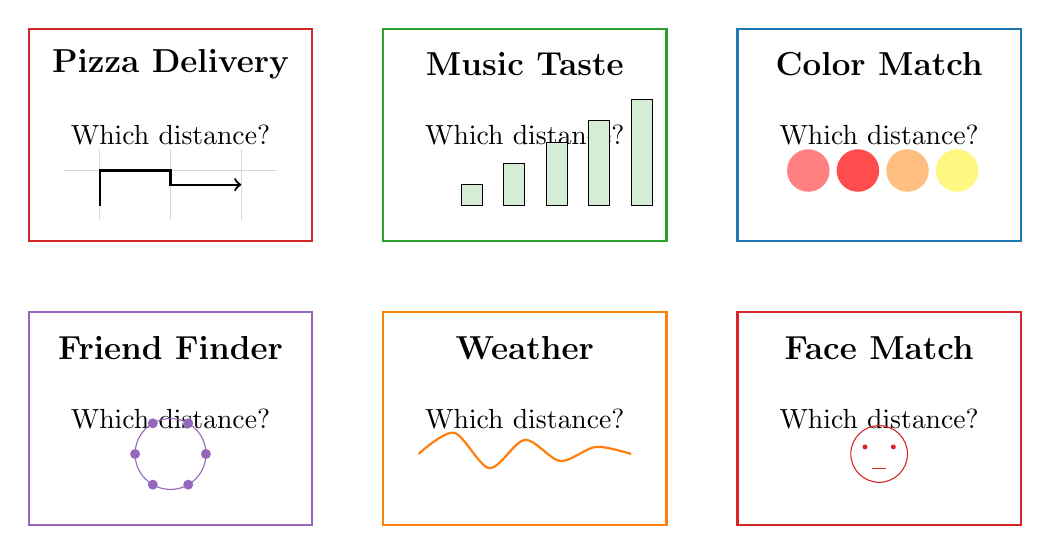
\begin{tikzpicture}[scale=0.9]
% Pizza delivery
\draw[thick, mlred] (0,4) rectangle (4,7);
\node[font=\large\bfseries] at (2,6.5) {Pizza Delivery};
\node at (2,5.5) {Which distance?};
\draw[gray!30] (0.5,4.3) grid (3.5,5.3);
\draw[thick, ->] (1,4.5) -- (1,5) -- (2,5) -- (2,4.8) -- (3,4.8);

% Music similarity
\draw[thick, mlgreen] (5,4) rectangle (9,7);
\node[font=\large\bfseries] at (7,6.5) {Music Taste};
\node at (7,5.5) {Which distance?};
\foreach \i in {1,...,5} {
    \draw[fill=mlgreen!20] (5.5+\i*0.6,4.5) rectangle (5.8+\i*0.6,4.5+\i*0.3);
}

% Color matching
\draw[thick, mlblue] (10,4) rectangle (14,7);
\node[font=\large\bfseries] at (12,6.5) {Color Match};
\node at (12,5.5) {Which distance?};
\fill[red!50] (11,5) circle (0.3);
\fill[red!70] (11.7,5) circle (0.3);
\fill[orange!50] (12.4,5) circle (0.3);
\fill[yellow!50] (13.1,5) circle (0.3);

% Friend recommendations
\draw[thick, mlpurple] (0,0) rectangle (4,3);
\node[font=\large\bfseries] at (2,2.5) {Friend Finder};
\node at (2,1.5) {Which distance?};
\foreach \angle in {0,60,120,180,240,300} {
    \fill[mlpurple] (2,1) ++(\angle:0.5) circle (2pt);
}
\draw[mlpurple] (2,1) circle (0.5);

% Weather patterns
\draw[thick, mlorange] (5,0) rectangle (9,3);
\node[font=\large\bfseries] at (7,2.5) {Weather};
\node at (7,1.5) {Which distance?};
\draw[mlorange, thick] plot[smooth] coordinates {(5.5,1) (6,1.3) (6.5,0.8) (7,1.2) (7.5,0.9) (8,1.1) (8.5,1)};

% Face recognition
\draw[thick, mlred] (10,0) rectangle (14,3);
\node[font=\large\bfseries] at (12,2.5) {Face Match};
\node at (12,1.5) {Which distance?};
\draw[mlred] (12,1) circle (0.4);
\fill[mlred] (11.8,1.1) circle (1pt);
\fill[mlred] (12.2,1.1) circle (1pt);
\draw[mlred] (11.9,0.8) -- (12.1,0.8);
\end{tikzpicture}
\end{center}

\vspace{2em}

\section*{Discovery Challenge}

\begin{center}
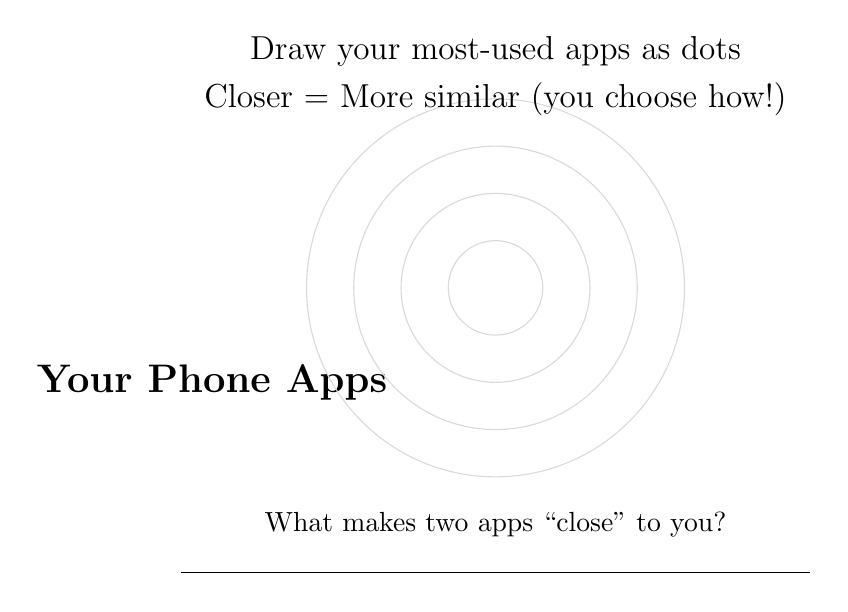
\begin{tikzpicture}[scale=1.2]
\node[font=\Large\bfseries] at (0,0) {Your Phone Apps};
\draw[gray!30] (3,1) circle (2);
\draw[gray!30] (3,1) circle (1.5);
\draw[gray!30] (3,1) circle (1);
\draw[gray!30] (3,1) circle (0.5);

\node at (3,3.5) {\large Draw your most-used apps as dots};
\node at (3,3) {\large Closer = More similar (you choose how!)};

\node at (3,-1.5) {What makes two apps ``close'' to you?};
\node at (3,-2) {\underline{\hspace{8cm}}};
\end{tikzpicture}
\end{center}

\vspace{2em}

\begin{tcolorbox}[colback=mlpurple!10, colframe=mlpurple!50]
\centering\large
\textbf{Next Class:} How ML picks the right distance automatically
\end{tcolorbox}

\end{document}